\chapter{Methodology}
\label{ch:methodology}
\begin{figure}[h]
	\centering
	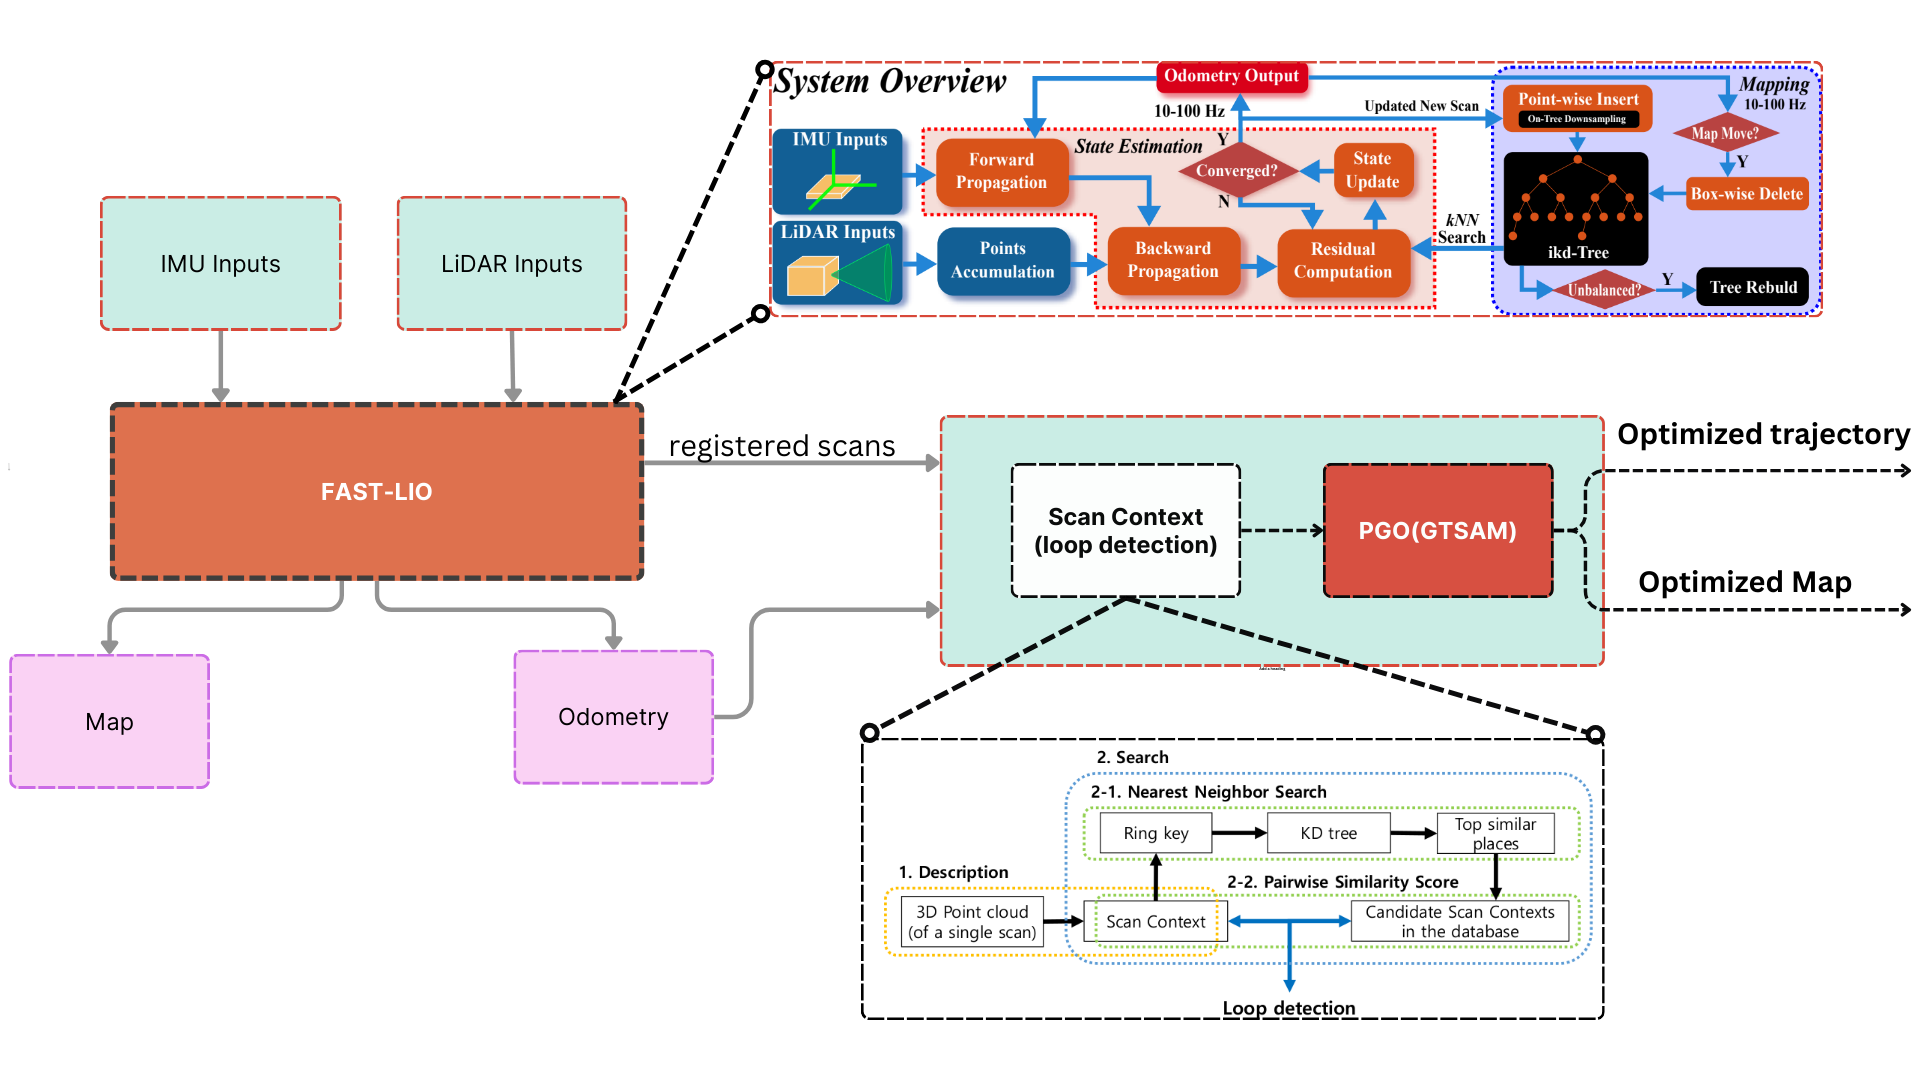
\includegraphics[width=\textwidth]{images/block-diagram.png}
	\caption{System overview of FAST-LIO with loop closure detection and optimization.}
	\label{fig:fast_lio}
\end{figure}

\section{System Overview}
The diagram illustrates a LiDAR-based FAST-LIO mapping system with loop closure detection and pose graph optimization. The key components include:

\begin{itemize}
	\item \textbf{FAST-LIO}: This module integrates IMU and LiDAR data to estimate the system's state in real time. It employs forward propagation for state prediction and backward propagation for refinement. Point cloud data is accumulated and processed using kNN search and residual computation to update the system state. The odometry output is generated at 10-100 Hz, while mapping is performed using an ikd-Tree for efficient point-wise insertion and deletion.
	\item \textbf{Scan Context}: This block is responsible for detecting loop closures by comparing newly acquired scans with previously stored scan contexts. It involves two main steps: (1) Nearest Neighbor Search, where a KD-tree and ring key are used to retrieve the most similar scan locations, and (2) Pairwise Similarity Score computation, which evaluates the resemblance between scan contexts to identify loop closures.
	\item \textbf{PGO (GTSAM)}: Optimizes the detected loop closures to refine the trajectory and map.
	\item The final output is an optimized trajectory and an improved map representation.
\end{itemize}
% Hardware

% Datasets


% LiDAR

% GNSS

% RTK
